\documentclass[11pt]{article}

\usepackage[a4paper,margin=2.5cm]{geometry}
\usepackage{amsmath,amssymb}
\usepackage{graphicx}
\usepackage[hidelinks]{hyperref}
\usepackage{booktabs}
\usepackage{enumitem}
\usepackage{xcolor}
\usepackage{caption}
\usepackage{float}

\title{\textbf{Domain Randomization for Sim-to-Sim Transfer}}
\author{Panagiotis Kiousis \and Emmanouil Tsiknakis}
\date{June 22, 2025}

\begin{document}
\maketitle

\begin{center}
\emph{Intelligent Control --- Course Project}
\end{center}

\vspace{0.3cm}
\noindent\textit{This is an extended, English-language version of the original Greek course report
(submitted June 22, 2025). It covers the same project and results, with additional derivations and
clarifications added where the original left things informal.}

\tableofcontents
\newpage

\section{Introduction}

This project implements and evaluates a reinforcement learning (RL) agent acting in a continuous,
two-dimensional environment. The agent's task is to learn to navigate efficiently towards a goal whose
position changes between episodes.

The central goal of the work is to train a policy in a simulated environment whose physical parameters
are randomized --- mass, friction, sensor noise, and the goal's position --- in order to study how well
the learned policy generalizes to new, unseen parameter settings. Evaluation focuses specifically on
\emph{zero-shot transfer}: whether the trained policy can cope with conditions it never encountered
during training, without any further fine-tuning.

The problem is addressed with Proximal Policy Optimization (PPO), one of the most widely used and
reliable policy-gradient methods. The agent is implemented as an Actor--Critic neural network, which
predicts both the policy (the distribution over actions) and an estimate of the state value.

The environment was built entirely from scratch, without relying on existing RL-environment libraries,
and includes realistic physical characteristics such as mass, friction, and a simulated LiDAR-type
sensor. Particular care was given to both functionality and visual rendering (2D and 3D), so that the
agent's behaviour could be inspected and analyzed directly.

\section{Domain Randomization}

Domain randomization is a technique used primarily in reinforcement learning and robotics to improve an
agent's generalization. The core idea is to inject deliberate randomness into the training environment:
every episode is run with different physical parameters, such as mass, friction, the goal's position,
sensor noise level, or even a different obstacle layout.

In this way, the agent is trained across a wide variety of scenarios instead of adapting to a single,
fixed, constrained environment. This improves robustness and allows the policy to cope satisfactorily
even with situations it has never seen before (zero-shot generalization).

The technique is especially valuable when there is a gap between simulation and the real world (the
\emph{sim-to-real gap}): by randomizing the simulated domain, the policy trained in simulation is more
likely to transfer successfully to real-world conditions, where the true parameters are uncertain or
variable.

In this project, domain randomization was applied to the agent's mass, its friction coefficient, the
goal's layout, and the characteristics of the LiDAR-type sensor. This strengthened the policy's ability
to operate reliably under different, unpredictable conditions.

\section{Environment}

\subsection{Environment Initialization}

At initialization, the environment defines the core state and action spaces, together with the physical
characteristics governing the agent's dynamics. The environment is continuous and two-dimensional, with
the agent moving on the $xy$-plane, within the range $[-10,10]\times[-10,10]$.

The observation space includes both physical and geometric parameters: specifically, the relative
position of the goal (obtained via the simulated LiDAR), the agent's mass, and its friction coefficient.

The agent's action is defined as a two-dimensional force that can be applied in any direction. The
magnitude of this force is bounded so that it stays within physically reasonable limits; this design
gives the learned policy more flexibility compared to a discrete action space.

The goal's initial position is randomized, while the agent always starts from the origin. The choice of
specific parameters --- mass, friction, and the timestep $\Delta t$ --- uses realistic physical
magnitudes and forms the basis for the domain randomization applied later, at each call to
\texttt{reset()}.

Finally, initialization also prepares the variables needed for 2D visualization of the environment,
allowing the agent's progress to be monitored as training proceeds (Figure~\ref{fig:env_init}).

\begin{figure}[H]
  \centering
  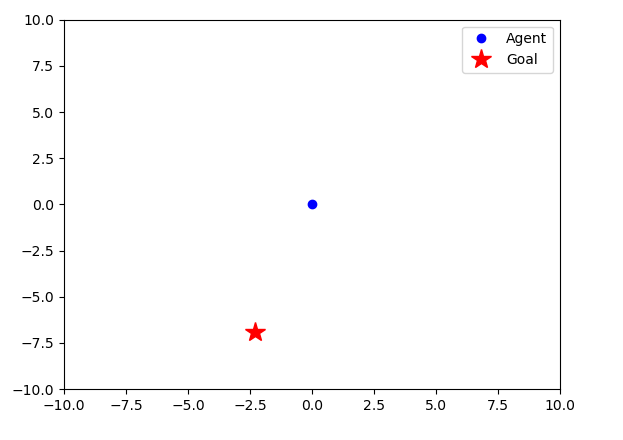
\includegraphics[width=0.6\textwidth]{figures/env_init.png}
  \caption{Initial state of the environment: the agent (blue) starts at the origin, the goal (red star)
  is placed at a randomized position within the $[-10,10]\times[-10,10]$ workspace.}
  \label{fig:env_init}
\end{figure}

\subsection{Dynamics}

The system takes as input the force applied to the agent. The next state of the system is computed in
the \texttt{compute\_dynamics} function, which implements the basic laws of dynamics to determine the
agent's new position and velocity:

\begin{align}
\text{Direction of the velocity vector:} \qquad & \hat{\mathbf{d}} = \frac{\mathbf{v}}{\lVert\mathbf{v}\rVert + 10^{-8}} \\[4pt]
\text{Friction force:} \qquad & \mathbf{f}_{\text{friction}} = -\,\text{friction}\cdot\hat{\mathbf{d}} \\[4pt]
\text{Acceleration:} \qquad & \mathbf{a} = \frac{\mathbf{F} + \mathbf{f}_{\text{friction}}}{m} \\[4pt]
\text{Velocity update:} \qquad & \mathbf{v}_{\text{new}} = \mathbf{v} + \mathbf{a}\cdot\Delta t \\[4pt]
\text{Position update:} \qquad & \mathbf{x}_{\text{new}} = \mathbf{x} + \mathbf{v}\cdot\Delta t + \tfrac{1}{2}\mathbf{a}\cdot\Delta t^{2}
\end{align}

where \texttt{friction} denotes the magnitude of the friction coefficient and $m$ the agent's mass. The
small constant $10^{-8}$ in the direction term avoids division by zero when the agent is at rest. This is
a standard semi-implicit Euler integration scheme: friction is modeled as a constant-magnitude force
opposing the current direction of motion (Coulomb-type friction), rather than a velocity-proportional
drag term.

\subsection{Goal Detection}

For added realism, the agent is assumed not to know the goal's position directly; instead, it is
equipped with a LiDAR-type sensor that scans the surrounding space.

The \texttt{lidar} function simulates the operation of a 2D LiDAR. Its purpose is to detect and measure
the distance and bearing angle to fixed reference points (in this setup, only the goal) relative to the
agent's position. To better simulate a real measuring device, Gaussian noise is added to the
measurements.

For each landmark, if the distance is smaller than a maximum range (\texttt{max\_range}), the detection
is recorded. The result is a list of detections, each containing the distance, the angle, and the ID of
the corresponding landmark:
\begin{align}
d_{\text{noisy}} &= d + \mathcal{N}(0,\sigma^2) \\
\theta_{\text{noisy}} &= \theta + \mathcal{N}(0,\sigma^2)
\end{align}
where $d=\lVert(m_x,m_y)-(p_x,p_y)\rVert$ and $\theta=\operatorname{atan2}(m_y-p_y,\,m_x-p_x)$ are the
noise-free distance and bearing to a landmark at $(m_x,m_y)$ from the agent's position $(p_x,p_y)$.

\subsection{Reward Computation}

The reward signal is a critical component for successfully training the agent, as it shapes the learned
behaviour towards the desired direction. The implemented reward function combines three main terms:

\begin{description}
  \item[Negative distance term.] The main driving term is the negative distance to the goal
  ($-\,\text{distance}$), which continuously encourages the agent to reduce its Euclidean distance to
  the destination. This term provides steady guidance towards the correct direction.
  \item[Directional alignment term.] To promote efficient navigation, the reward is boosted by a positive
  term computed as the inner product between the normalized action and the normalized direction towards
  the goal. This term takes values in $[-1,1]$ and rewards actions that are aligned with the desired
  direction of motion.
  \item[Success bonus.] When the agent comes within the goal's critical radius (the \texttt{threshold}),
  it receives a substantial bonus of $+100$. This signals successful completion of the episode and
  reinforces the behaviour that led to it.
\end{description}

Written out explicitly, with $\hat{\mathbf{a}}$ the normalized action and $\hat{\mathbf{g}}$ the
normalized direction towards the goal:
\begin{equation}
r = -\,\lVert \mathbf{p}_{\text{goal}} - \mathbf{p}_{\text{agent}} \rVert
    \;+\; 10\,\bigl(\hat{\mathbf{a}}\cdot\hat{\mathbf{g}}\bigr)
    \;+\; \mathbf{1}\!\left[\lVert \mathbf{p}_{\text{goal}} - \mathbf{p}_{\text{agent}} \rVert < \text{threshold}\right]\cdot 100 .
\label{eq:reward}
\end{equation}
This closed form was not written out explicitly in the original report, which described the three terms
only in words; Equation~\eqref{eq:reward} is added here for precision, and matches exactly what
\texttt{compute\_reward} computes in \texttt{env.py}.

\subsection{Agent--Environment Interaction}

The \texttt{step} function implements the core logic of the agent's interaction with the environment at
each timestep. Specifically, it takes an action (a force) as input and returns the observation, the
reward, and a flag indicating episode termination (\texttt{done}).

First, the action is clipped to the allowed range. The resulting force is then passed to
\texttt{compute\_dynamics} to update the agent's position and velocity, accounting for the system's
physics. The position is clipped so that it stays within the predefined workspace bounds.

Next, the LiDAR sensor is triggered to detect the goal. If a valid detection occurs, the distance and
angle to the goal are extracted and converted to Cartesian components $(dx, dy)$. These, together with
the agent's physical parameters (mass and friction), make up the observation vector returned to the
agent.

Immediately afterward, the reward is computed via \texttt{compute\_reward}, as described above. The
episode terminates either when the agent reaches the goal or when the maximum number of steps is
exhausted.

\subsection{3D Visualization}

To monitor the agent's training, a 3D visualization system was implemented using the \texttt{pygame} and
\texttt{OpenGL} libraries.

The function \texttt{init\_pygame\_3d()} creates a $1000\times800$ window with OpenGL support. A
perspective projection is applied (field of view $45^{\circ}$, depth range $0.1$--$100$), and the camera
is positioned so that the two-dimensional plane is viewed as a 3D "scene."

Lighting is enabled via \texttt{GL\_LIGHT0}, with the light source placed at $(10,10,20)$ and configured
ambient, diffuse, and specular parameters. Objects are given materials with appropriate reflectivity and
shininess properties for a more realistic appearance.

A space-themed background is loaded with \texttt{pygame} and converted into an OpenGL texture. It is
rendered by \texttt{draw\_background()}, which uses an orthographic projection and temporarily disables
lighting and depth testing (Figure~\ref{fig:intro_render} shows this background, together with the agent
and goal rendered as cylinders on the ground plane).

\begin{figure}[H]
  \centering
  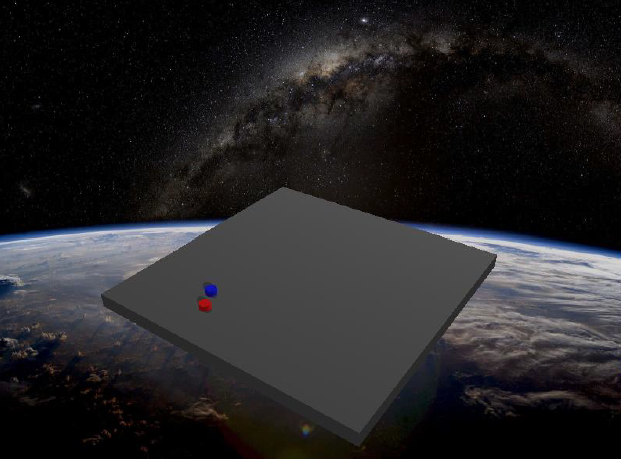
\includegraphics[width=0.75\textwidth]{figures/intro_render.png}
  \caption{3D visualization of the environment: the ground plane is rendered as a platform against a
  space-themed background, with the agent and goal shown as colored cylinders.}
  \label{fig:intro_render}
\end{figure}

The environment includes:
\begin{itemize}
  \item \textbf{Ground.} \texttt{draw\_ground()} builds a ground plane with extent $[-10,10]$ and a
  height of 1 unit, from quads with correctly oriented normal vectors.
  \item \textbf{Cylinders.} The agent and the goal are each rendered as a cylinder of radius and height
  $0.4$, via \texttt{draw\_cylinder()} and the GLU library.
\end{itemize}

\texttt{draw\_shadow()} creates semi-transparent shadows, rendered as gray disks slightly above the
ground plane to avoid z-fighting. Each object is given distinct material properties:
\begin{itemize}
  \item \textbf{Agent:} blue $(0.1, 0.1, 1.0)$, shininess $50.0$.
  \item \textbf{Goal:} red $(1.0, 0.1, 0.1)$, shininess $30.0$.
  \item \textbf{Ground:} gray-blue $(0.3, 0.35, 0.45)$, shininess $10.0$.
\end{itemize}

\texttt{render\_3d()} brings all of this together: clearing the buffers, drawing the background, the
ground, the shadows, and the objects, and finally updating the display buffer with a refresh period of
$10\,\text{ms}$. In the training loop, this visualization is only triggered during the final 5\% of
training epochs (every 5 steps), so as not to slow down the bulk of training.

\section{Neural Network Architecture}

\subsection{Actor--Critic Model}

To solve the navigation problem, an Actor--Critic architecture was adopted, which combines the
advantages of value-based methods and policy-based methods. The model consists of shared layers and two
specialized heads: the \emph{Actor}, which produces the policy's action, and the \emph{Critic}, which
estimates the state's value.

The shared architecture consists of a linear layer mapping the observation (\texttt{obs\_dim}~$=4$) to a
64-dimensional representation, followed by a $\tanh$ non-linearity. This shared representation serves
both policy learning and value estimation.

The Actor consists of two linear layers with an intermediate $\tanh$ activation, producing logits for
the two action dimensions (\texttt{act\_dim}~$=2$). The Actor's output is used as the mean of a Normal
distribution that models the policy's action. The Critic follows a similar structure, producing a single
value representing the long-term expected return (the estimated value of the current state).

\begin{equation}
h = \tanh(W_1 o + b_1), \qquad
\mu = W_{a2}\bigl(\tanh(W_{a1} h + b_{a1})\bigr) + b_{a2}, \qquad
V(s) = W_{c2}\bigl(\tanh(W_{c1} h + b_{c1})\bigr) + b_{c2},
\end{equation}
where $o\in\mathbb{R}^{4}$ is the observation, $h\in\mathbb{R}^{64}$ the shared representation, $\mu$ the
mean of the action distribution and $V(s)$ the Critic's value estimate.

\subsection{Observation Space}

The observation vector was designed to give the agent the information needed for effective navigation.
Specifically, it consists of four dimensions:
\begin{itemize}
  \item \textbf{Relative goal position $(dx, dy)$.} The Cartesian components of the relative goal
  position, obtained by converting the LiDAR's polar measurements: $dx = d\cos\theta$,
  $dy = d\sin\theta$.
  \item \textbf{Agent mass.} Affects the system's dynamic behaviour according to the laws of motion;
  including it lets the agent adapt its strategy to its own physical characteristics.
  \item \textbf{Friction coefficient.} Determines the resistance to motion, affecting the agent's dynamic
  response to applied forces.
\end{itemize}

The choice of this compact observation space follows the principle of minimizing complexity while
retaining the necessary information. Rather than providing the absolute coordinates of the agent and the
goal directly, the relative position offers translation invariance, while the physical parameterization
allows the policy to adapt to different dynamic conditions.

\section{Training with Proximal Policy Optimization (PPO)}

\subsection{PPO Algorithm and Parameters}

To train the Actor--Critic model, the Proximal Policy Optimization (PPO) algorithm was chosen, which
combines the advantages of trust-region methods with simplicity of implementation, using clipping on the
policy ratio to avoid excessively large updates.

Two configurations were trained and compared in this project, differing only in the total number of
epochs (see Section~\ref{sec:results}):

\begin{itemize}
  \item \textbf{Learning rate:} $1\times10^{-4}$, with exponential decay (a \texttt{StepLR} scheduler,
  $\gamma=0.8$ every 10 epochs)
  \item \textbf{Steps per epoch:} 1024 interaction steps per epoch
  \item \textbf{Mini-batch size:} 64 samples per mini-batch
  \item \textbf{Clip epsilon:} $0.1$, for clipping the policy ratio
  \item \textbf{Discount factor ($\gamma$):} $0.99$, used when computing returns
  \item \textbf{GAE $\lambda$:} $0.95$, for Generalized Advantage Estimation
  \item \textbf{Total epochs:} 100 in the first configuration, 200 in the second.
\end{itemize}

\subsection{Dynamic Exploration Schedule}

An important feature of the implementation is the dynamic adjustment of exploration during training. The
standard deviation of the action distribution decreases linearly from $0.5$ at the start of training to
$0.1$ at the end, according to:
\begin{equation}
\sigma = \sigma_{\text{initial}} - \bigl(\sigma_{\text{initial}} - \sigma_{\text{final}}\bigr)\cdot
\frac{\text{epoch}}{\text{total\_epochs}}.
\end{equation}
This schedule allows the agent to explore the action space extensively in the early stages, while
gradually "trusting" the network's output more as the policy evolves and improves.

\subsection{Training Loop and Data Collection}

During the main training loop, the agent interacts with the environment for 1024 steps per epoch,
collecting trajectories of experience. During this phase, the following are stored:
\begin{itemize}
  \item \textbf{Observations} (\texttt{obs\_buf}): the environment states.
  \item \textbf{Actions} (\texttt{act\_buf}): the agent's selected actions.
  \item \textbf{Log-probabilities} (\texttt{logp\_buf}): the actions' probabilities under the policy that
  collected them.
  \item \textbf{Value estimates} (\texttt{val\_buf}): the Critic's predictions.
  \item \textbf{Rewards} (\texttt{rew\_buf}): the rewards received.
  \item \textbf{Done flags} (\texttt{done\_buf}): the episode-termination indicators.
\end{itemize}
Data collection is accompanied by a success counter (\texttt{success\_count}), incremented whenever the
agent reaches within the goal's critical radius.

\subsection{Returns and Advantage Estimation}

Once the data has been collected, returns are computed using the Generalized Advantage Estimation (GAE)
algorithm. GAE is a technique that addresses the classic bias--variance trade-off in advantage
estimation:
\begin{itemize}
  \item \textbf{Monte Carlo returns:} high variance, low bias.
  \item \textbf{Temporal-Difference (TD) methods:} low variance, higher bias.
  \item \textbf{GAE:} combines both approaches through a parameter $\lambda$ ($\lambda=1$ corresponds to
  MC, $\lambda=0$ to TD).
\end{itemize}

For each timestep, a TD error (\(\delta\)) is computed, expressing the discrepancy between the actual
reward received and the model's prediction:
\begin{equation}
\delta_t = r_t + \gamma\, V(s_{t+1})\,(1-d_t) - V(s_t),
\end{equation}
where $d_t = 1$ if the episode terminated at step $t$ (\texttt{done}), and $0$ otherwise (so that the
bootstrap term vanishes at an episode boundary, correctly reducing to $\delta_t = r_t - V(s_t)$).

GAE then uses this error with exponential smoothing (via the hyperparameters $\gamma$ and $\lambda$) to
produce the final advantage estimate, computed recursively backward from the end of the trajectory to its
start:
\begin{equation}
\hat{A}_t = \delta_t + \gamma\lambda(1-d_t)\,\hat{A}_{t+1}.
\end{equation}
Unrolling the recursion gives the equivalent, more commonly cited closed form as a weighted sum of future
TD errors (added here as a complement to the recursive definition in the original report):
\begin{equation}
\hat{A}_t = \sum_{l=0}^{T-t-1} (\gamma\lambda)^{l}\,\delta_{t+l}.
\end{equation}
The returns used as the Critic's regression target are then:
\begin{equation}
\text{return}_t = \hat{A}_t + V(s_t).
\end{equation}
Advantages are normalized by subtracting their mean and dividing by their standard deviation, a technique
that improves training stability and accelerates convergence:
\begin{equation}
\hat{A}_t \leftarrow \frac{\hat{A}_t - \text{mean}(\hat{A})}{\text{std}(\hat{A}) + \varepsilon}.
\end{equation}

\subsection{Policy Update with PPO}

Training is driven by the advantage, which expresses the discrepancy between the return actually achieved
and the value predicted by the Critic. A positive advantage means the outcome was better than expected,
so the agent should reinforce that action's probability; a negative advantage implies underperformance,
so the action's probability should be reduced.

PPO implements these updates while avoiding large changes that could destabilize training. To this end,
it first computes the probability ratio between the new and the old policy:
\begin{equation}
\text{ratio} = \frac{\pi_{\text{new}}(a\mid s)}{\pi_{\text{old}}(a\mid s)} = \exp\bigl(\log\pi_{\text{new}} - \log\pi_{\text{old}}\bigr).
\end{equation}
This ratio shows how much the action's probability has changed: a ratio $>1$ means the new policy
considers the action more likely, while a ratio $<1$ means less likely.

The \textbf{PPO clipped objective} uses two versions of the surrogate loss:
\begin{align}
\text{surrogate}_1 &= \text{ratio}\cdot \hat{A}, \\
\text{surrogate}_2 &= \operatorname{clip}(\text{ratio},\, 1-\varepsilon,\, 1+\varepsilon)\cdot \hat{A}.
\end{align}

During training, the experience gathered from the rollout is shuffled randomly and split into mini-batches
of size 64. The update is applied on each mini-batch and repeated 10 times per epoch to achieve stable
convergence. In each such pass, three loss terms are computed:

\textbf{Policy loss:}
\begin{equation}
L_{\text{policy}} = -\min(\text{surrogate}_1,\, \text{surrogate}_2).
\end{equation}
The negative sign is used because the network minimizes its loss, i.e.\ it maximizes the surrogate
objective (reinforcing good actions). Hence, the more negative the policy loss, the better the policy
update is considered to be.

\textbf{Value loss:} the mean squared error between the value estimates and the computed returns,
\begin{equation}
L_{\text{value}} = \frac{1}{N}\sum_{i=1}^{N}\bigl(\text{return}_i - V(s_i)\bigr)^2.
\end{equation}

\textbf{Entropy:} measures the policy's uncertainty. High entropy means the policy spreads probability
roughly uniformly across the available actions, while low entropy indicates decisiveness and reduced
exploration. Encouraging entropy prevents premature convergence to local optima, promoting more resilient
behaviour, especially in the early stages of training.

The total loss combines the three terms:
\begin{equation}
L = L_{\text{policy}} + 0.5\, L_{\text{value}} - 0.01\, \mathcal{H},
\end{equation}
where $\mathcal{H}$ denotes the policy's entropy. This procedure embodies the core principles of
policy-gradient methods, offering a way to update the policy with a view toward both stability and
training effectiveness.

\subsection{Progress Monitoring and Early Stopping}

Training is carried out over multiple epochs and monitored via the mean reward per epoch. An early
stopping mechanism is implemented, with patience equal to 25\% of the total number of epochs (50 epochs
in the 200-epoch configuration). Whenever a new best model is detected, its state dictionary is saved for
later use.

During the final 5\% of epochs, the 3D visualization is enabled every 5 steps, allowing visual inspection
of the trained agent's behaviour. Training ends either when all epochs are completed or when early
stopping is triggered, ensuring efficient use of computational resources and helping to avoid overfitting.

Figure~\ref{fig:training_log} shows an excerpt of the console output during one of the training runs,
illustrating how the average reward per epoch evolves and when new best models are found.

\begin{figure}[H]
  \centering
  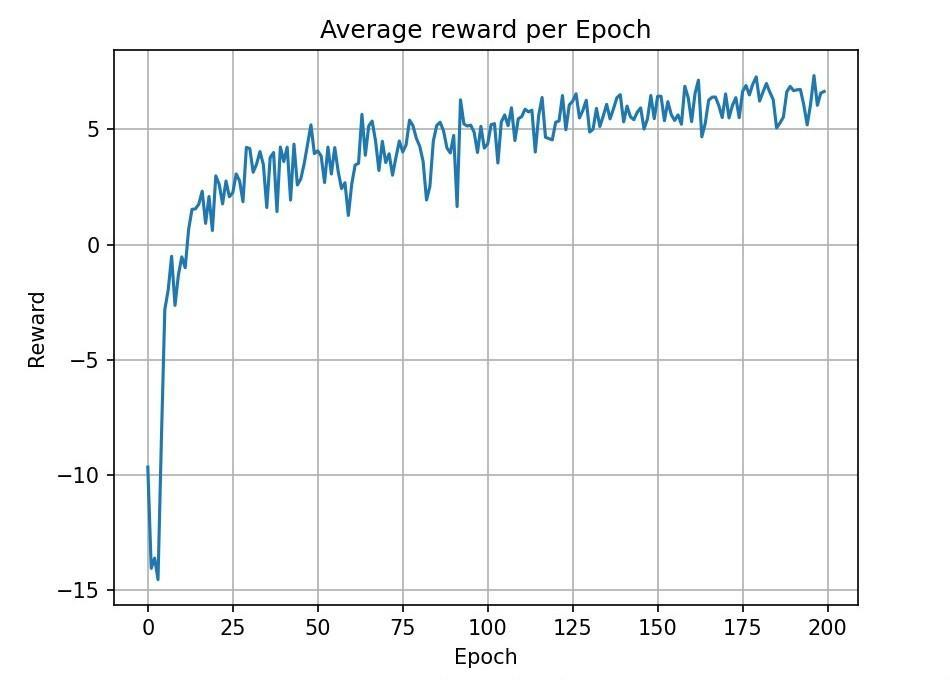
\includegraphics[width=0.55\textwidth]{figures/training_log.png}
  \caption{Console output during training: the average reward per epoch, with new best models flagged as
  they are found.}
  \label{fig:training_log}
\end{figure}

\section{Results}
\label{sec:results}

As shown in the corresponding plots, the agent's policy improves progressively over the course of
training. Figure~\ref{fig:rewards} shows the evolution of the mean reward per epoch for the two trained
configurations. A clear improvement trend is visible during training, with rewards stabilizing at
positive values after the first 20--40 epochs, indicating that the agent has learned to approach its
goal effectively.

\begin{figure}[H]
  \centering
  \begin{minipage}{0.48\textwidth}
    \centering
    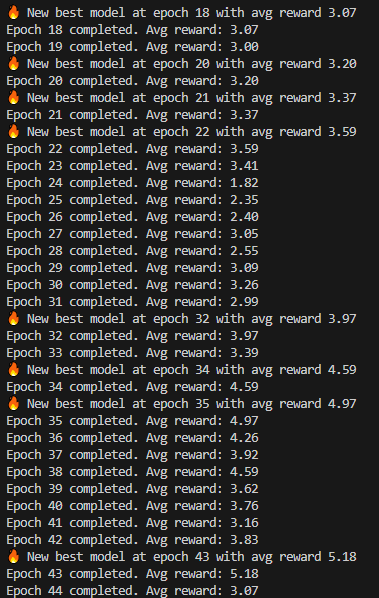
\includegraphics[width=\textwidth]{figures/reward_100.png}
    \caption*{100 epochs}
  \end{minipage}\hfill
  \begin{minipage}{0.48\textwidth}
    \centering
    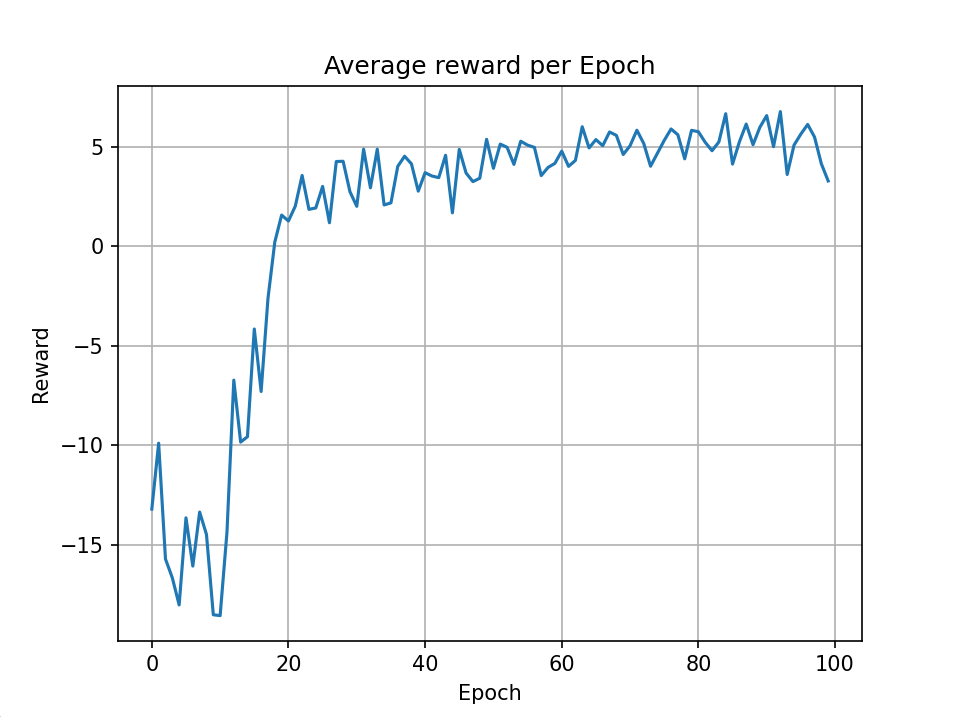
\includegraphics[width=\textwidth]{figures/reward_200.png}
    \caption*{200 epochs}
  \end{minipage}
  \caption{Average reward per epoch for the 100-epoch and 200-epoch training configurations.}
  \label{fig:rewards}
\end{figure}

After training, the best policy model is evaluated on 10 environments with randomized parameters, to
assess zero-shot transfer. As shown in Figure~\ref{fig:zeroshot}, both policies perform quite well (a
high success rate), with the second model, trained for 200 epochs, reaching a 100\% success rate.

\begin{figure}[H]
  \centering
  \begin{minipage}{0.48\textwidth}
    \centering
    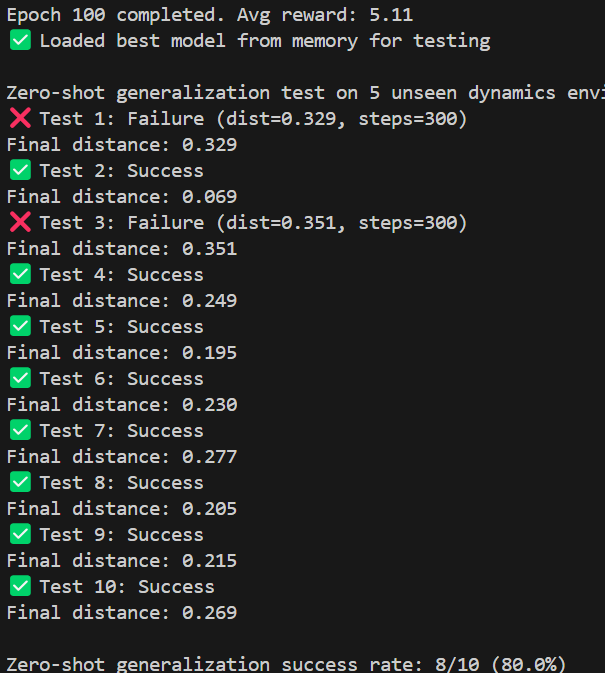
\includegraphics[width=\textwidth]{figures/zeroshot_100.png}
    \caption*{100-epoch model: 8/10 (80\%)}
  \end{minipage}\hfill
  \begin{minipage}{0.48\textwidth}
    \centering
    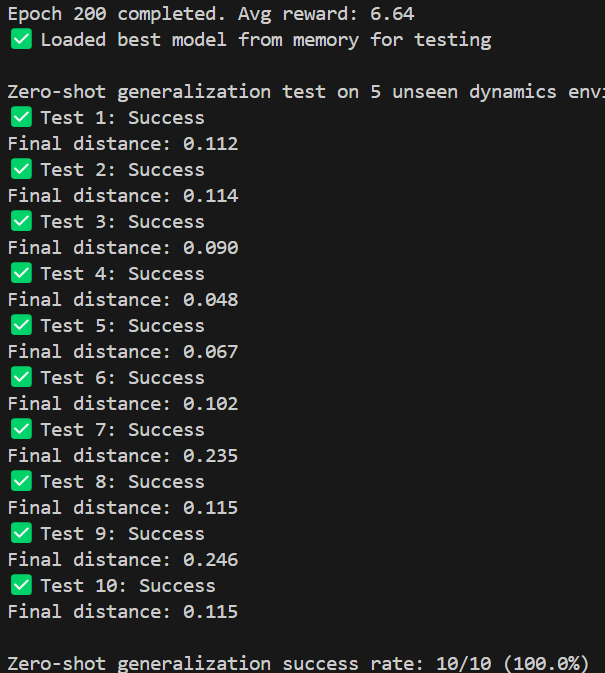
\includegraphics[width=\textwidth]{figures/zeroshot_200.png}
    \caption*{200-epoch model: 10/10 (100\%)}
  \end{minipage}
  \caption{Zero-shot generalization test on 10 unseen, randomized environments.}
  \label{fig:zeroshot}
\end{figure}

Figure~\ref{fig:trajectories} shows the results of the test runs in the two-dimensional environment.
Agents that reached the goal within the threshold distance ($=0.3$) are shown in blue, while those that
did not are shown in red; the final goal position is also shown for each test.

\begin{figure}[H]
  \centering
  \begin{minipage}{0.48\textwidth}
    \centering
    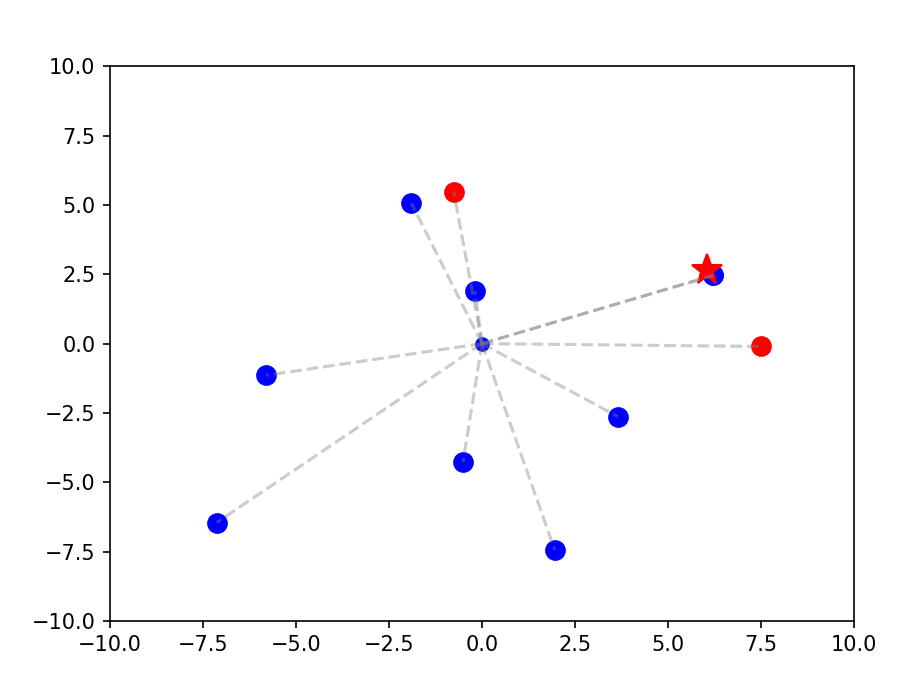
\includegraphics[width=\textwidth]{figures/trajectories_100.png}
    \caption*{100-epoch model (2 failures, shown in red)}
  \end{minipage}\hfill
  \begin{minipage}{0.48\textwidth}
    \centering
    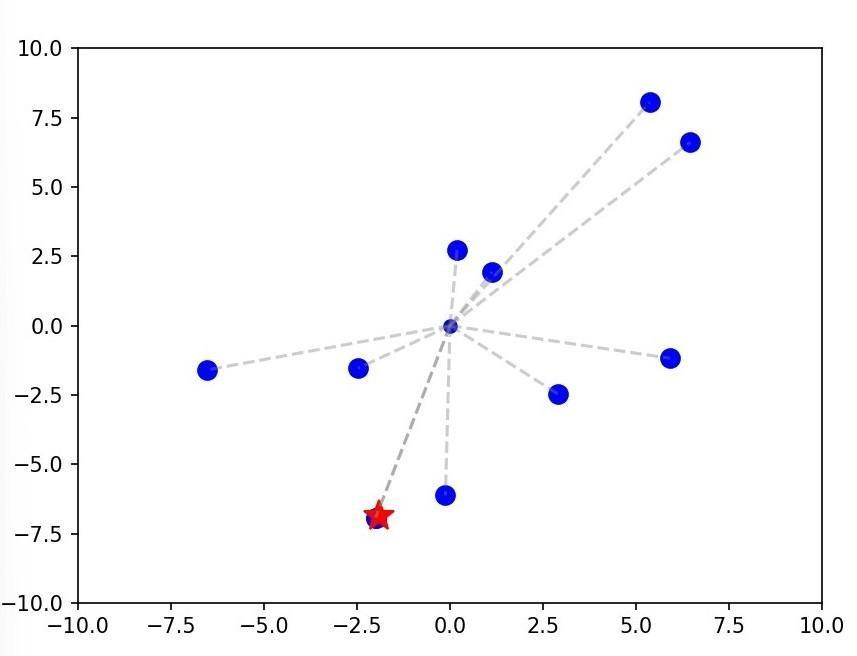
\includegraphics[width=\textwidth]{figures/trajectories_200.png}
    \caption*{200-epoch model (all successes)}
  \end{minipage}
  \caption{Final agent positions across the 10 zero-shot test environments, relative to each episode's
  goal.}
  \label{fig:trajectories}
\end{figure}

These results show that the policy managed to learn a navigation strategy that is stable and effective,
even in randomized environments it had never encountered. The success on the zero-shot tests demonstrates
that domain randomization contributed substantially to the agent's generalization, and that the
additional 100 epochs of training (200 vs.\ 100) translated into a tangible, measurable improvement in
zero-shot robustness (80\% $\to$ 100\% success, and a reduction in the final distance-to-goal spread
across the successful runs).

\section{Conclusion}

This project implemented a complete sim-to-sim domain randomization pipeline for a 2D navigation task,
from the physics and sensor simulation up through a PPO-trained Actor--Critic policy and a 3D
visualization layer, all built without relying on an existing RL-environment framework. Randomizing mass,
friction, and goal placement at each episode reset, combined with a compact, translation-invariant
observation space, produced a policy that transfers in a zero-shot setting to previously unseen dynamics
with a high success rate, and that success rate improves further with additional training. The main
practical takeaway is that even a fairly simple domain-randomization scheme, applied to just a handful of
physical parameters, is enough to produce meaningfully robust zero-shot generalization in this setting.

\section{Sources}

\begin{enumerate}
  \item Tobin, J., Fong, R., Ray, A., Schneider, J., Zaremba, W., and Abbeel, P. (2017, September).
  Domain randomization for transferring deep neural networks from simulation to the real world. In
  \emph{2017 IEEE/RSJ International Conference on Intelligent Robots and Systems (IROS)} (pp.~23--30).
  \item Schulman, J., Wolski, F., Dhariwal, P., Radford, A., \& Klimov, O. (2017). \emph{Proximal Policy
  Optimization Algorithms}. arXiv preprint arXiv:1707.06347.
  \href{https://arxiv.org/abs/1707.06347}{https://arxiv.org/abs/1707.06347}
  \item Weng, L. (2018). Policy Gradient Algorithms.
  \href{https://lilianweng.github.io/posts/2018-04-08-policy-gradient/}{lilianweng.github.io/posts/2018-04-08-policy-gradient}
  \item Course lecture slides (Intelligent Control).
  \item ChatGPT was used for supporting research while documenting this project (as noted in the original
  Greek report).
\end{enumerate}

\end{document}
